\chapter{Methodology}

 \begin{figure*}[htbp]
    \centering
    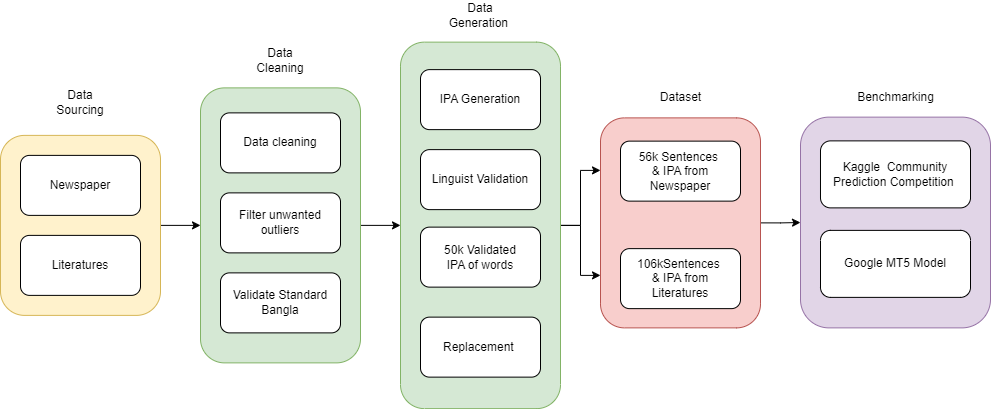
\includegraphics[width=\textwidth]{Images/Diagram/methodology.png}
    \caption{Workflow Diagram of the whole Project}
    \label{fig:wrokflow}
\end{figure*} 


The realm of Bangla IPA transcription has long awaited a comprehensive and robust dataset to fuel advancements in research and applications. In this work, we proudly present the DUAL-IPA dataset, a pioneering resource meticulously crafted to address this need. Standing as the first-of-its-kind large-scale dataset specifically designed for Bangla IPA, DUAL-IPA sets a new benchmark for quality, diversity, and accessibility.

This chapter meticulously documents the journey of constructing DUAL-IPA, encompassing every step from data collection and expert annotation to comprehensive statistical analysis. We unveil the intricate processes involved in sourcing diverse Bangla sentences, harnessing the expertise of linguists for accurate IPA transcription, and streamlining the annotation workflow through innovative techniques. Furthermore, we delve into the dataset's statistical composition, offering valuable insights into its vocabulary breadth, sentence length distribution, and phoneme landscape. Through this in-depth exploration, we not only illuminate the characteristics of DUAL-IPA, but also demonstrate its immense potential to empower researchers and practitioners in the field of Bangla NLP. 

\section{Data Collection and Preparation}
\subsection{Data Sources}
\begin{itemize}
    \item Data were collected from newspapers, online platforms, e-books.
    \item We wanted to make sure we cover all the conventional sources of standard Bangla for both word and sentence level that we use in our daily life.
\end{itemize}
\subsection{Data Scraping Techniques}
\begin{itemize}
    \item To scrape all these data, we wrote multiple python scripts specific to each source.
    \item As different platform and formats have different data structures and most of them are not in a standard format when scraped, we had to study the data types first properly in order to find patterns so that we can maximize our output in terms of number and quality.
\end{itemize}

\subsection{Data Cleaning and Preprocessing}
\begin{itemize}
    \item Removing duplicates, irrelevant content, and noise.
    \item Addressing missing values with justification.
    \item Language identification and filtering for non-promito bangla contents.
\end{itemize}

\section{IPA Transcription Process}
We were given a few words and IPA. We constructed a simple septa graph to identify unique phonemes. Using these phonemes and septa graph we made a Jupiter notebook that can generate IPA given a word. The notebook generates 116 IPAs.



\subsection{Word-Level Transcription}
Using this notebook, we generated around 50k IPAs for 50k unique words from 56k sentences provided by Bengali.AI These sentences were taken from newspapers.

\subsection{Sentence-Level Transcription}
We generated around 162k IPA from online sources and e-books after a rigorous process of collecting and cleaning the data. Then, using the same model as the word-level data, 162k IPA was generated for the 162k sentences.


\section{Linguistic Review and Adjustments}
\begin{itemize}
    \item After every transcription, a team of linguists from University of Dhaka thoroughly reviewed each word and sentence to make sure they are on par with the standard rules and regulation.
    \item Then, based on the feedbacks of the linguists, changes were made to the data to make sure the dataset it as accurate as possible.
    \item There were some debate about some transcriptions, that were mitigated by taking opinion from \textbf{Professor Dr. Syed Shahrier Rahman from Department of Linguistics, University of Dhaka}, who also led the team of linguists for this project.
\end{itemize}

\section{Dataset Creation and Finalization}
\begin{itemize}
    \item  The final dataset is \textbf{two CSV} file, one for newspaper sentence IPA transcription and one for Literature sentence IPA transcription, containing two columns which are: sentences, clean\_validated\_ipa sentences, IPA.
    \item The whole dataset contains 160,000+ Bengali words and sentences with their corresponding IPAs.
    \item we have chosen to open-source the DUAL-IPA dataset under the \textbf{CC BY-SA 4.0 license}, making it freely accessible to researchers and practitioners worldwide.
\end{itemize}

\section{Achievements}
Through this work, we achieved
\begin{itemize}
    \item 160,000+ word and sentence level dataset for Bengali to IPA transcription.
    \item Human and Machine Validation of the dataset.
    \item Arrange a national level competition on the dataset in collaboration with \textbf{IIT Software Engineers’ Community (IITSEC), University of Dhaka}, where this dataset was put into test and different models were created based on it.
    \item Submitting our paper in the prestigious \textbf{LREC-Coling - 2024 conference}.
\end{itemize}
